\subsection{Record user behavior}
\label{sec:inputdata}

\begin{figure}
  \centering
     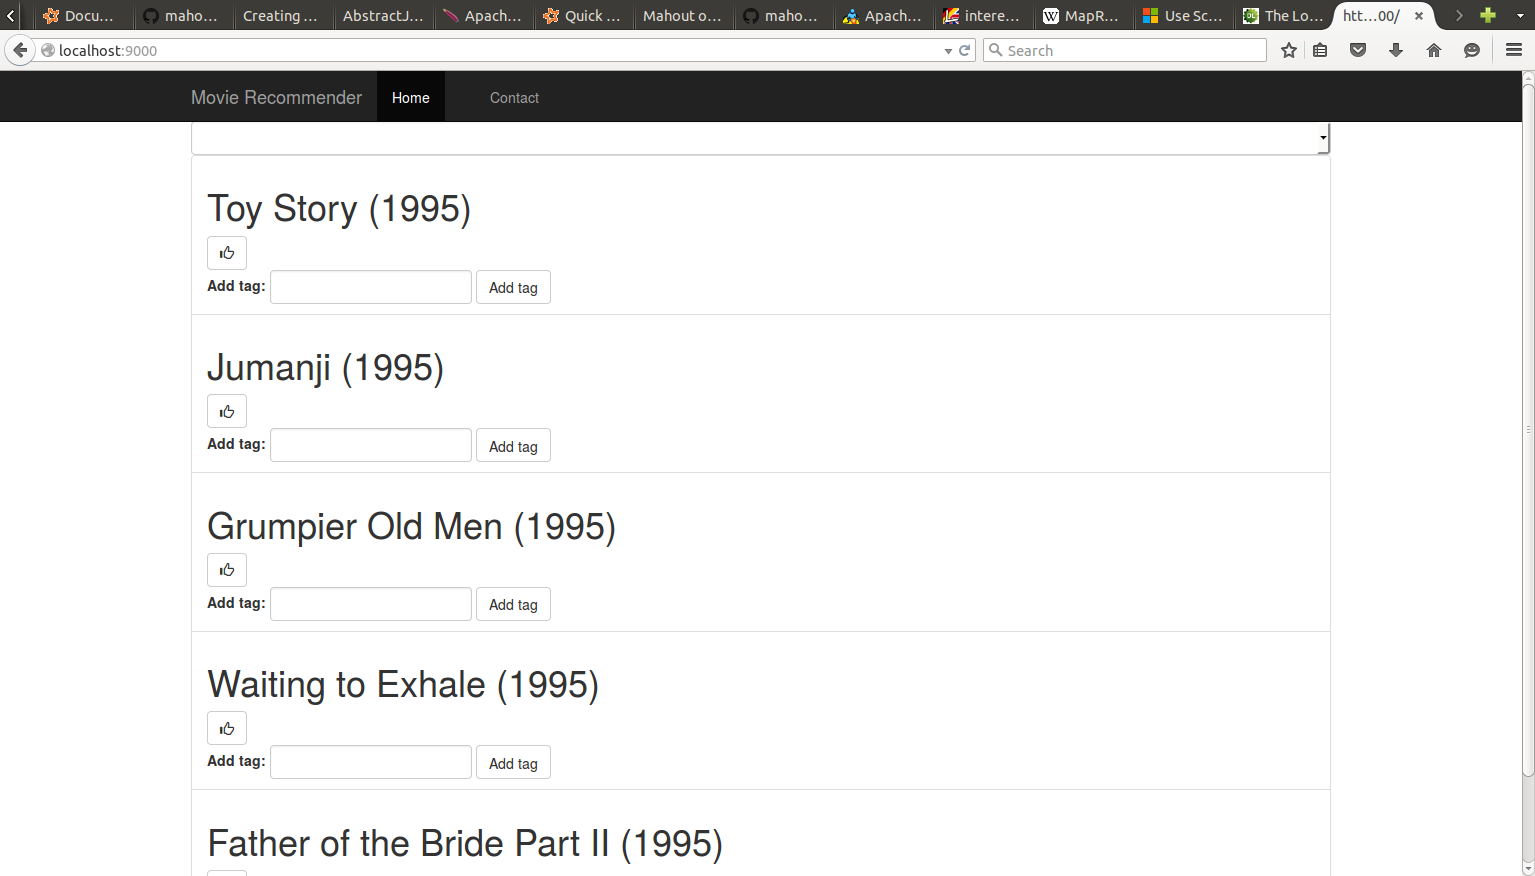
\includegraphics[width=0.9\textwidth]{collectinginput}
  \caption{The user can like and tag movies with the web front end. The user actions are recorded by the web server.}
  \label{fig:gui}
\end{figure}

Many collaborative filtering recommender engines use explicit user ratings to train their model. Explicit user ratings of a user for an item are expressed by numbers (e.g. a rating is a number between 1 and 5). The use of explicit feedback has some drawbacks.
\begin{itemize}
\item Only a small subset of users will rate items. This leads to a model that is skewed against user who like to rate.
\item The majority of ratings are associated with a small fraction of the most popular items \cite{Anderson}. As a result it is less likely that unknown items show up in the \gls{topn}. This behavior is undesirable because the goal of the recommender is to present items the a user would not find on his own.
\end{itemize}

Corresponding to \cite{Dunning14} the best choice of input data is the collection of past user actions on a website. The stored behavior of one user is called the user's \gls{history}. The history records what users actually do. Hence the input data should consist of recorded \glspl{useraction} (e.g. purchase, view, like, tag).

In our demo web application we record two different user actions:
\begin{description}
\item[like]  Users can express their positive feedback for a movie by clicking on a ``like'' button (the \gls{like} action is an explicit rating. We use it instead of a purchase or view action in order to keep the GUI simple).
\item[tag] User can \gls{tag} items. Every item can be associated with a list of \glspl{tag}.
\end{description}
The recorded like and tag action are later used to compute similarity between items.
Figure \ref{fig:gui} shows the simplistic user interface of our demo web app.

The web browser sends every user action to the web server. The web server provides a REST Web API that receives the \glspl{useraction} as HTTP \verb|Post| request and saves them to a sqlite3 \footnote{https://www.sqlite.org/} database.

In order to analyze the data later we want to retrieve the action history $h_u$ for a particular user $u$ for a defined action and a list of tags for every item. Hence we have to structure the data accordingly. Figure \ref{fig:er} shows the entity relationship diagram for the user actions \gls{like} and \gls{tag}

\tikzset{multi  attribute/.style={attribute ,double  distance=1.5pt}}
\tikzset{derived  attribute/.style={attribute ,dashed}}
\tikzset{total/.style={double  distance=1.5pt}}
\tikzset{every  entity/.style={draw=blue , fill=blue!20}}
\tikzset{every  attribute/.style={draw=yellow, fill=yellow!20, node distance=1.0cm}}
\tikzset{every  relationship/.style={draw=red, fill=red!20}}

\begin{figure}
\centering
\begin{tikzpicture}[node distance=2.0cm]
  \node[entity](user){user};
  \node[relationship](like)[above right of=user]{ like } edge (user);
  \node[attribute](date2)[above of=like]{ date } edge (like);
  \node[entity](item)[below right of=like]{item} edge (like);
  \node[relationship](tag)[below right of=user]{ tag } edge (user) edge (item);
  \node[attribute](text)[below right of=tag]{ text } edge (tag);
  \node[attribute](date1)[below left of=tag]{ date } edge (tag);
  \end{tikzpicture}
\caption{The data model allows us to retrieve the action history for every user. Like and tag form associations of user with item.}
\label{fig:er}
\end{figure}

It makes sense to start recording behavioral data month's before deploying the recommender engine because the recommender engine has to analyze the data and build a model of similarity among items in order to create personalized recommendations.

